%(BEGIN_QUESTION)
% Copyright 2007, Tony R. Kuphaldt, released under the Creative Commons Attribution License (v 1.0)
% This means you may do almost anything with this work of mine, so long as you give me proper credit

Identifiser hvilke av disse ventilhusene som er {\it direktevirkende}, og hvilke som er {\it reversvirkende}:

$$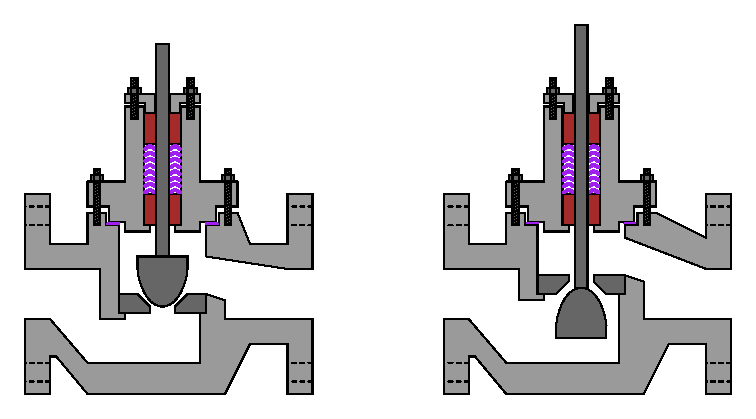
\includegraphics[width=15.5cm]{i01629x01.eps}$$

Identifiser på samme måte hvilke av disse ventilaktuatorene som er {\it direktevirkende}, og hvilke som er {\it reversvirkende}:

$$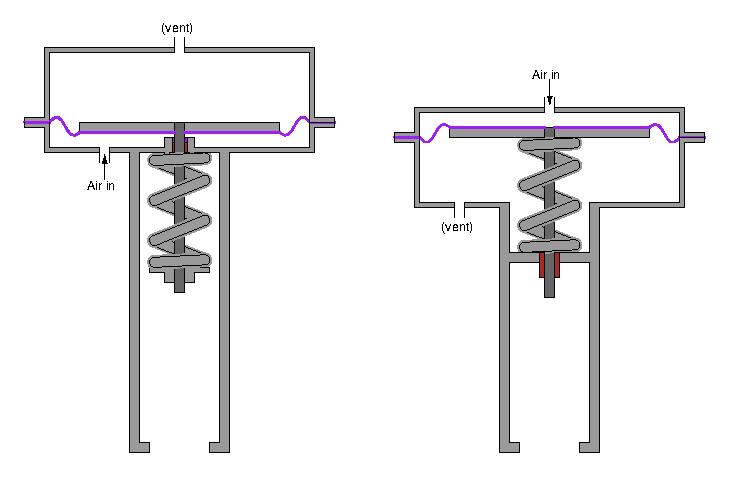
\includegraphics[width=15.5cm]{i01629x02.eps}$$

Til slutt: identifiser {\it to kombinasjoner} av ventilhus og aktuatorer som gir en {\it air-to-close}-ventil.

\underbar{file i01629}
%(END_QUESTION)





%(BEGIN_ANSWER)

Jeg anbefaler 2 poeng for korrekt identifikasjon av ventiltypene, 2 poeng for korrekt identifikasjon av aktuatortypene, og 3 poeng for hver korrekt kombinasjon av ventil/aktuator (totalt 10 poeng).

$$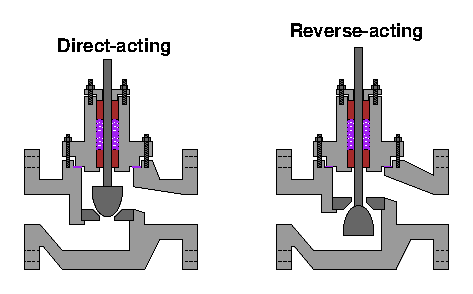
\includegraphics[width=15.5cm]{i01629x03.eps}$$

$$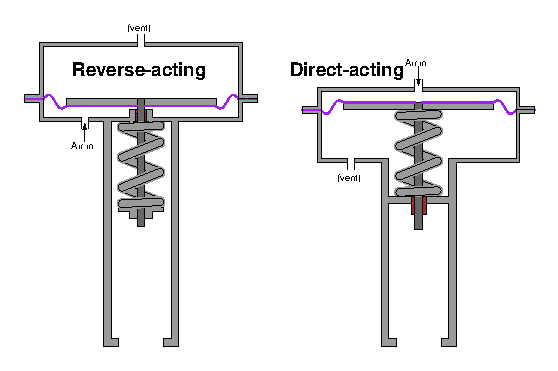
\includegraphics[width=15.5cm]{i01629x04.eps}$$

For en air-to-close-ventil, kombiner en {\it direktevirkende ventil og direktevirkende aktuator}, eller kombiner en {\it reversvirkende ventil og reversvirkende aktuator}.

%(END_ANSWER)





%(BEGIN_NOTES)

{\bf Dette spørsmålet er kun ment for eksamen, ikke arbeidsark!}.

%(END_NOTES)
